\chapter{Signed curvature}
\label{chap:signed-curvature}

\section{Definitions}\label{sec:def(skur)}

Suppose $\gamma$ is a smooth unit-speed plane curve,
so $\tan(s)=\gamma'(s)$ is its unit tangent vector for any $s$.

Let us rotate $\tan(s)$ by the angle $\tfrac\pi 2$ counterclockwise; 
denote the obtained vector by $\norm(s)$.
The pair $\tan(s),\norm(s)$ is an oriented orthonormal frame in the plane which is analogous to the Frenet frame
defined in Section~\ref{sec:frenet-frame};
we will keep the name \index{Frenet frame}\emph{Frenet frame} for it.

Recall that $\gamma''(s)\perp \gamma'(s)$ (see \ref{prop:a'-pertp-a''}).
Therefore 
\[\tan'(s)=\skur(s)\cdot \norm(s).\eqlbl{eq:tau'}\]\index{10k@$\skur$}
for some real number $\skur(s)$;
the value $\skur(s)$ is called \index{signed curvature}\emph{signed curvature} of $\gamma$ at $s$.
We may use notation $\skur(s)_\gamma$ if we need to specify the curve~$\gamma$.

Note that 
\[\kur(s)=|\skur(s)|;\]
that is, up to sign, the signed curvature $\skur(s)$ equals the curvature $\kur(s)$  of $\gamma$ at $s$ defined in Section~\ref{sec:curvature};
the sign tells us in which direction $\gamma$ turns --- if $\gamma$ is turning left at time $s$, then $\skur (s)>0$.
If we want to emphasise that we are working with the {}\emph{non-signed} curvature of the curve, 
we call it \index{absolute curvature}\emph{absolute curvature}.

Note that if we reverse the parametrization of $\gamma$ or change the orientation of the plane, then
the signed curvature changes its sign.

Since $\tan(s),\norm(s)$ is an orthonormal frame, we have 
\begin{align*}
\langle\tan,\tan\rangle&=1,
&
\langle\norm,\norm\rangle&=1, 
&
\langle\tan,\norm\rangle&=0,
\end{align*}
Differentiating these identities we get 
\begin{align*}
\langle\tan',\tan\rangle&=0,
&
\langle\norm',\norm\rangle&=0,
&
\langle\tan',\norm\rangle+\langle\tan,\norm'\rangle&=0,
\end{align*}
By \ref{eq:tau'}, $\langle\tan',\norm\rangle=\skur$ and therefore $\langle\tan,\norm'\rangle=-\skur$.
Hence we get 
\[\norm'(s)=-\skur(s)\cdot \tan(s).\eqlbl{eq:nu'}\]
The equations \ref{eq:tau'} and \ref{eq:nu'} are the Frenet formulas for plane curves. 
They can be written in matrix form as:
\[
\begin{pmatrix}
\tan'
\\
\norm'
\end{pmatrix}
=
\begin{pmatrix}
0&\skur
\\
-\skur&0
\end{pmatrix}
\cdot
\begin{pmatrix}
\tan
\\
\norm
\end{pmatrix}.
\]

\begin{thm}{Exercise}\label{ex:bike}
Let $\gamma_0\:[a,b]\to\RR^2$ be a smooth regular curve and $\tan$ its tangent indicatrix.
Consider another curve $\gamma_1\:[a,b]\to\RR^2$ defined by $\gamma_1(t)=\gamma_0(t)+\tan(t)$.
Show that
\[\length\gamma_0\le \length\gamma_1.\]

\end{thm}

The curves $\gamma_0$ and $\gamma_1$ in the exercise above describe the tracks of an idealized bicycle with  distance 1 from the rear to the front wheel.
Thus by the exercise, the front wheel must have a longer track.
For more on the geometry of bicycle tracks, see the survey of Robert Foote, Mark Levi, and Serge Tabachnikov \cite{foote-levi-tabachnikov} and the references therein.

\section{Fundamental theorem of plane curves}

\begin{thm}{Theorem}\label{thm:fund-curves-2D}
Let $\skur(s)$ be a smooth real valued function defined on a real interval $\mathbb{I}$.
Then there is a smooth unit-speed curve $\gamma\:\mathbb{I}\to\RR^2$ with signed curvature $\skur(s)$.
Moreover, $\gamma$ is uniquely defined up to a rigid motion of the plane.
\end{thm}

This is the fundamental theorem of plane curves; it is a direct analog of \ref{thm:fund-curves} and it can be proved along the same lines.
We present a slightly simpler proof.
\parit{Proof.} 
Fix $s_0\in\mathbb{I}$.
Consider the function
\[\theta(s)
=
\int_{s_0}^s\skur(t)\cdot dt.\]
Note that by the fundamental theorem of calculus, we have $\theta'(s)\z=\skur(s)$ for all~$s$.

Set 
\[\tan(s)=(\cos[\theta(s)],\sin[\theta(s)])\] and let $\norm(s)$ be its counterclockwise rotation by angle $\tfrac\pi2$; so 
\[\norm(s)=(-\sin[\theta(s)],\cos[\theta(s)]).\]
Consider the curve 
\[\gamma(s)=\int_{s_0}^s\tan(s)\cdot ds.\]
Since $|\gamma'|=|\tan|=1$, the curve $\gamma$ is unit-speed and $\tan,\norm$ is its Frenet frame. 

Note that
\begin{align*}
\gamma''(s)&=\tan'(s)=
\\
&=(\cos[\theta(s)]',\sin[\theta(s)]')=
\\
&=\theta'(s)\cdot (-\sin[\theta(s)],\cos[\theta(s)])=
\\
&=\skur(s)\cdot \norm(s).
\end{align*}
So $\skur(s)$ is the signed curvature of $\gamma$ at $s$. 

This proves the existence;
it remains to prove the uniqueness.

Assume $\gamma_1$ and $\gamma_2$ are two curves that satisfy the assumptions of the theorem.
Applying a rigid motion, we can assume that $\gamma_1(s_0)\z=\gamma_2(s_0)\z=0$ and the Frenet frame of both curves at $s_0$ is formed by the coordinate frame $(1,0),(0,1)$.
Let us denote by $\tan_1,\norm_1$ and $\tan_2,\norm_2$ the Frenet frames of $\gamma_1$ and $\gamma_2$ respectively.
Both triples $\gamma_i,\tan_i,\norm_i$ satisfy the following system of ordinary differential equations 
\[
\begin{cases}
\gamma_i'=\tan_i,
\\
\tan_i'=\skur\cdot\norm_i,
\\
\norm_i'=-\skur\cdot\tan_i.
\end{cases}
\]

Moreover, they have the same initial values at $s_0$.
By the uniqueness of solutions of ordinary differential equations (\ref{thm:ODE}), we have $\gamma_1=\gamma_2$.
\qeds

Note that from the proof of the theorem we obtain the following corollary:



\begin{thm}{Corollary}\label{cor:2D-angle}
Let $\gamma\:\mathbb{I}\to\RR^2$ be a smooth unit-speed curve and $s_0\z\in \mathbb{I}$.
Denote by $\skur$ the signed curvature of $\gamma$.
Assume an oriented $(x,y)$-coordinate system is chosen in such a way that $\gamma(s_0)$ is the origin and $\gamma'(s_0)$ points in the direction of the $x$-axis.
Then 
\[\gamma'(s)=(\cos[\theta(s)],\sin[\theta(s)]) , \]
for all $s$, where 
\[\theta(s)=\int_{s_0}^s\skur(t)\cdot dt.\]
\end{thm}


\section{Total signed curvature}

Let $\gamma\:\mathbb{I}\to\RR^2$ be a smooth unit-speed plane curve.
The \index{total signed curvature}\emph{total signed curvature} of $\gamma$, denoted by $\tgc\gamma$, is defined as the integral
\[\tgc\gamma
=
\int_\mathbb{I} \skur(s)\cdot ds,\eqlbl{eq:tsc-k}\]\index{10psi@$\tgc\gamma$}
where $\skur$ denotes the signed curvature of $\gamma$.

Note that if $\mathbb{I}=[a,b]$, then 
\[\tgc\gamma=\theta(b)-\theta(a),\eqlbl{eq:tsc-theta}\]
where $\theta$ is as in \ref{cor:2D-angle}.

If $\gamma$ is a piecewise smooth and regular plane curve, then we define its total signed curvature as the sum of the total signed curvatures of its arcs plus the sum of the \emph{signed} external angles at its joints;
they are positive where $\gamma$ turns left, negative where $\gamma$ turns right, and 0 where $\gamma$ goes straight.
It is undefined if it turns exactly backward;
that is, if the curve has a cusp.
That is, if $\gamma$ is a concatenation of smooth and regular arcs $\gamma_1,\dots,\gamma_n$, then 
\[\tgc\gamma=\tgc{\gamma_1}+\dots+\tgc{\gamma_n}+\theta_1+\dots+\theta_{n-1}\]
where $\theta_i$ is the signed external angle at the joint between $\gamma_i$ and $\gamma_{i+1}$.
If $\gamma$ is closed, then the concatenation is cyclic and
\[\tgc\gamma=\tgc{\gamma_1}+\dots+\tgc{\gamma_n}+\theta_1+\dots+\theta_{n},\]
where $\theta_n$ is the signed external angle at the joint between $\gamma_n$ and $\gamma_1$.

Since $\left|\int \skur(s)\cdot ds\right|\le \int|\skur(s)|\cdot ds$, we have
\[|\tgc\gamma|\le \tc\gamma\eqlbl{eq:tsc-tc}\] 
for any smooth regular plane curve $\gamma$;
that is, the total signed curvature $\tgc{}$ cannot exceed the total curvature $\tc{}$ in absolute value.
Note that the equality holds if and only if the signed curvature does not change sign.

\begin{thm}{Exercise}\label{ex:trochoids}
A trochoid is a curve traced out by a point fixed to a wheel as it rolls along a straight line.
\begin{figure}[h!]
\centering
\begin{lpic}[t(-0mm),b(0mm),r(0mm),l(0mm)]{asy/trochoids}
\lbl[l]{4,0;{\footnotesize $-\tfrac32$}}
\lbl[l]{4,6;{\footnotesize $-1$}}
\lbl[tl]{10,15;{\footnotesize $-\tfrac12$}}
\lbl[t]{22,17;{\footnotesize $0$}}
\lbl[r]{3,23.6;{\footnotesize $\tfrac12$}}
\lbl[r]{3,29.4;{\footnotesize $1$}}
\lbl[r]{3,35.2;{\footnotesize $\tfrac32$}}

\end{lpic}
\end{figure}
A family of \index{trochoid}\emph{trochoids} $\gamma_a\:[0,2\cdot\pi]\to \RR^2$ (see the picture) can be parametrized as
\[\gamma_a(t)=(t+a\cdot \sin t, a\cdot \cos t).\]
\begin{enumerate}[(a)]
\item Given $a\in \RR$, find $\tgc{\gamma_a}$ if it is defined.
\item Given $a\in \RR$, find $\tc{\gamma_a}$.
\end{enumerate}
\end{thm}

\begin{thm}{Proposition}\label{prop:total-signed-curvature}
Any closed simple smooth regular plane curve $\gamma$ has total signed curvature  $\pm2\cdot\pi$; it is $+2\cdot\pi$
if the region bounded by $\gamma$ lies on the left from it and  $-2\cdot\pi$ otherwise.

Moreover the same statement holds for any closed piecewise simple smooth regular plane curve $\gamma$ if its total signed curvature is defined.
\end{thm}

This proposition is called sometimes \index{Umlaufsatz}\emph{Umlaufsatz}; it is a differential-geometric analog of the theorem about the sum of the internal angles of a polygon (\ref{thm:sum=(n-2)pi}) which we use in the proof.
A more conceptual proof was given by Heinz Hopf \cite{hopf1935}, \cite[p. 42]{hopf1989}.

\parit{Proof.}
Without loss of generality we may assume that $\gamma$ is oriented in such a way that the region bounded by $\gamma$ lies on the left from it.
We can also assume that it is parametrized by arc-length.

Consider a closed polygonal line $\beta=p_1\dots p_n$ inscribed in $\gamma$.
We can assume that the arcs between the vertexes are sufficiently small 
so that the polygonal line is simple and each arc $\gamma_i$ from $p_i$ to $p_{i+1}$ has small total absolute curvature, say  $\tc{\gamma_i}<\pi$ for each $i$.

\begin{wrapfigure}[13]{o}{43 mm}
\vskip4mm
\centering
\includegraphics{mppics/pic-59}
\vskip4mm
\end{wrapfigure}

As usual we use indexes modulo $n$, in particular $p_{n+1}\z=p_1$.
Assume $p_i=\gamma(t_i)$.
Set 
\begin{align*}
\vec w_i&=p_{i+1}-p_i,& \vec v_i&=\gamma'(t_i),
\\
\alpha_i&=\measuredangle(\vec v_i,\vec w_i),&\beta_i&=\measuredangle(\vec w_{i-1},\vec v_i),
\end{align*}
where $\alpha_i,\beta_i\in(-\pi,\pi]$ are signed angles --- $\alpha_i$ is positive if $\vec w_i$ points to the left from $\vec v_i$.

By \ref{eq:tsc-theta}, the value
\[\tgc{\gamma_i}-\alpha_i-\beta_{i+1}\eqlbl{eq:Psi-alpha-beta}\]
is a multiple of $2\cdot\pi$.
Since $\tc{\gamma_i}<\pi$, by the chord lemma (\ref{lem:chord}), we also have that $|\alpha_i|\z+|\beta_i|<\pi$.
By \ref{eq:tsc-tc}, we have that $|\tgc{\gamma_i}|\le\tc{\gamma_i}$;
therefore the value in \ref{eq:Psi-alpha-beta} vanishes.
In other word,for each $i$ we have
\[\tgc{\gamma_i}=\alpha_i+\beta_{i+1}.\]

Note that 
\[\delta_i=\pi-\alpha_i-\beta_i\eqlbl{eq:delta=pi-alpha-beta}\] 
is the internal angle of $\beta$ at $p_i$;
$\delta_i\in (0,2\cdot\pi)$ for each $i$.
Recall that the sum of the internal angles of an $n$-gon is $(n-2)\cdot \pi$ (see \ref{thm:sum=(n-2)pi}); that is,
\[\delta_1+\dots+\delta_n=(n-2)\cdot \pi.\]
Therefore 
\[
\begin{aligned}
\tgc\gamma&=\tgc\gamma_1+\dots+\tgc\gamma_n=
\\
&=(\alpha_1+\beta_2)+\dots+(\alpha_n+\beta_1)=
\\
&=(\beta_1+\alpha_1)+\dots+(\beta_n+\alpha_n)=
\\
&=(\pi-\delta_1)+\dots+(\pi-\delta_n)=
\\
&=n\cdot\pi-(n-2)\cdot \pi=
\\
&=2\cdot\pi.
\end{aligned}\eqlbl{eq:delta=pi-alpha-beta-sum}\]

The case of piecewise smooth and regular curves is done the same way;
we need to subdivide the arcs in the cyclic concatenation further to meet the requirement above and instead of equation \ref{eq:delta=pi-alpha-beta} we have 
\[\delta_i=\pi-\alpha_i-\beta_i-\theta_i,\]
where $\theta_i$ is the signed external angle of $\gamma$ at $p_i$; it vanishes if the curve $\gamma$ is smooth at $p_i$.
Therefore instead of equation \ref{eq:delta=pi-alpha-beta-sum}, we have
\begin{align*}
\tgc\gamma&=\tgc{\gamma_1}+\dots+\tgc{\gamma_n}+\theta_1+\dots+\theta_n=
\\
&=(\alpha_1+\beta_2)+\dots+(\alpha_n+\beta_1)=
\\
&=(\beta_1+\alpha_1+\theta_1)+\dots+(\beta_n+\alpha_n+\theta_n)=
\\
&=(\pi-\delta_1)+\dots+(\pi-\delta_n)=
\\
&=n\cdot\pi-(n-2)\cdot \pi=
\\
&=2\cdot\pi.
\end{align*}
\qedsf

\begin{thm}{Exercise}\label{ex:zero-tsc}
Draw a smooth regular closed plane curve $\gamma$ such that 

\begin{subthm}{ex:zero-tsc:0}$\tgc\gamma=0$;
\end{subthm}
 
\begin{subthm}{ex:zero-tsc:5}$\tgc\gamma=\tc\gamma=10\cdot\pi$;
\end{subthm}

\begin{subthm}{ex:zero-tsc:2-4}$\tgc\gamma=2\cdot \pi$ and $\tc\gamma=4\cdot\pi$.
\end{subthm}

\end{thm}

\begin{thm}{Exercise}\label{ex:length'}
Let $\gamma\:[a,b]\to\RR$ be a smooth regular plane curve with Frenet frame $\tan,\norm$.
Given a real parameter $\ell$, consider
the curve $\gamma_\ell(t)\z=\gamma(t)+\ell\cdot\norm(t)$; it is called a {}\emph{parallel curve of $\gamma$ at signed distance~$\ell$}.

\begin{subthm}{ex:length':reg}
Show that $\gamma_\ell$ is a regular curve if $\ell\cdot \skur(t)\ne 1$ for all $t$, where $\skur(t)$ denotes the signed curvature of $\gamma$.
\end{subthm}
 
\begin{subthm}{ex:length':formula}
Set $L(\ell)=\length\gamma_\ell$.
Show that 
\[L(\ell)=L(0)-\ell\cdot\tgc\gamma\eqlbl{eq:length(parallel-curve)}\]
for all $\ell$ sufficiently close to $0$. 
\end{subthm}

\begin{subthm}{ex:length':antiformula}
Describe an example showing that formula \ref{eq:length(parallel-curve)} does not hold for all~$\ell$. 
\end{subthm}

\end{thm}


\section{Osculating circline}

\begin{thm}{Proposition}\label{prop:circline}
Given a point $p$,
a unit vector $\tan$ 
and a real number $\skur$, there is a unique smooth unit-speed curve $\sigma\:\RR\to\RR^2$ 
that starts at $p$ in the direction of $\tan$ and has constant signed curvature $\skur$.

Moreover, if $\skur=0$, then it is a line $\sigma(s)=p+s\cdot \tan$;
if $\skur\ne 0$, then $\sigma$ runs around a circle of radius $\tfrac1{|\skur|}$ with center at $p+\tfrac1\skur\cdot \norm$, where $\tan,\norm$ is an oriented orthonormal frame.
\end{thm}

Further we will use the term \index{circline}\emph{circline} for {}\emph{a circle or a line};
these are the only plane curves with constant signed curvature.

\parit{Proof.}
The proof is done by a calculation based on \ref{thm:fund-curves-2D} and \ref{cor:2D-angle}.

Suppose $s_0=0$, choose a coordinate system such that $p$ is its origin and $\tan$ points in the direction of the $x$-axis. Therefore $\norm$ points in the direction of the $y$-axis.
Then
\begin{align*}\theta(s)&=\int_{0}^s\skur\cdot dt=
\\
&=\skur\cdot s.
\end{align*}
Therefore
\[\sigma'(s)=(\cos[\skur\cdot s],\sin[\skur\cdot s]).\]
It remains to integrate the last identity.
If $\skur=0$, we get 
\[\sigma(s)=(s,0)\]
which describes the line $\sigma(s)=p+s\cdot \tan$.

If $\skur\ne 0$, we get
\[\sigma(s)=(\tfrac1\skur\cdot\sin[\skur\cdot s],
\tfrac1\skur\cdot(1-\cos[\skur\cdot s])).\]
which is the circle of radius $r=\tfrac1{|\skur|}$ centered at $(0,\tfrac1\skur)=p+\tfrac1\skur\cdot\norm$.
\qeds


\begin{wrapfigure}{r}{31 mm}
\vskip-0mm
\centering
\includegraphics{mppics/pic-21}
\vskip0mm
\end{wrapfigure}

\begin{thm}{Definition}
Let $\gamma$ be a smooth unit-speed plane curve;
denote by $\skur(s)$ the signed curvature of $\gamma$ at $s$.

The unit-speed curve $\sigma$ of constant signed curvature $\skur(s)$ that starts at $\gamma(s)$ in the direction $\gamma'(s)$ is called the \index{osculating!circline}\emph{osculating circline} of $\gamma$ at~$s$.

The center and radius of the osculating circle at a given point are called the \index{center of curvature}\emph{center of curvature} and \index{radius of curvature}\emph{radius of curvature} of the curve at that point.
\end{thm}

The osculating circle $\sigma_s$ can be also defined as the unique circline that has \index{order of contact}\emph{second order of contact} with $\gamma$ at $s$;
that is, $\rho(\ell)\z=o(\ell^2)$, where $\rho(\ell)$ denotes the distance from $\gamma(s+\ell)$ to $\sigma_s$.

The following exercise is recommended to the reader familiar with the notion of \index{inversion}\emph{inversion}.

\begin{thm}{Advanced exercise}\label{ex:inverse}
Suppose $\gamma$ is a smooth regular plane curve that does not pass thru the origin.
Let $\hat \gamma$ be the inversion of $\gamma$ with respect to the unit circle centered at the origin.
Show that the osculating circline of $\hat\gamma$ at $s$ is the inversion of the osculating circline of $\gamma$ at $s$.
\end{thm}

\section{Spiral lemma}
\label{spiral}

The following lemma was proved by Peter Tait \cite{tait}
and later rediscovered by Adolf Kneser \cite{kneser}.

\begin{wrapfigure}{r}{31 mm}
\vskip-4mm
\begin{lpic}[t(-0 mm),b(-2 mm),r(0 mm),l(0 mm)]{mppics/pic-61}
\end{lpic}
\end{wrapfigure}

\begin{thm}{Lemma}\label{lem:spiral}
Assume that $\gamma$ is a smooth regular plane curve with strictly decreasing positive signed curvature. Then the osculating circles of $\gamma$ are nested; that is, if $\sigma_s$ denoted the osculating circle of $\gamma$ at $s$,
then $\sigma_{s_0}$ lies in the open disc bounded by $\sigma_{s_1}$ for any $s_0<s_1$. \index{10sigma@$\sigma_s$}
\end{thm}

It turns out that the osculating circles of the curve $\gamma$ give a peculiar foliation of an annulus by circles; it has the following property: if a smooth function is constant on each osculating circle, then it must be constant in the annulus \cite[see][Lecture 10]{fuchs-tabachnikov}.
Also note that the curve $\gamma$ is tangent to a circle of the foliation at each of its points.
However, it does not run along any of those circles.

\parit{Proof.}
Let $\tan(s),\norm(s)$ be the Frenet frame,
$\omega(s)$, $r(s)$
the center and radius of curvature of $\gamma$.
By \ref{prop:circline},
\[\omega(s)=\gamma(s)+r(s)\cdot \norm(s).\]

\begin{wrapfigure}{o}{35 mm}
\vskip-0mm
\centering
\begin{lpic}[t(-0 mm),b(-0 mm),r(0 mm),l(0 mm)]{mppics/pic-84}
\end{lpic}
\end{wrapfigure}

Since $\skur>0$, we have that $r(s)\cdot\skur(s)=1$.
Therefore applying Frenet formula \ref{eq:nu'}, we get that
\begin{align*}
\omega'(s)&=\gamma'(s)+r'(s)\cdot \norm(s)+r(s)\cdot \norm'(s)=
\\
&=\tan(s)+r'(s)\cdot \norm(s)-r(s)\cdot \skur(s)\cdot \tan(s)=
\\
&=r'(s)\cdot \norm(s).
\end{align*}
Since $\skur(s)$ is decreasing, $r(s)$ is increasing;
therefore $r'\ge 0$.
It follows that $|\omega'(s)|= r'(s)$ and $\omega'(s)$ points in the direction of $\norm(s)$.

Since $\norm'(s)=-\skur(s)\cdot\tan(s)$, the direction of $\omega'(s)$ cannot have constant direction on a nontrivial interval;
that is, the curve $s\mapsto \omega(s)$ contains no line segments.
Therefore 
\begin{align*}
|\omega(s_1)-\omega(s_0)|&<\length(\omega|_{[s_0,s_1]})=
\\
&=\int_{s_0}^{s_1}|\omega'(s)|\cdot ds=
\\
&=\int_{s_0}^{s_1}r'(s)\cdot ds=
\\
&=r(s_1)-r(s_0).
\end{align*}

In other words, the distance between the centers of $\sigma_{s_1}$ and $\sigma_{s_0}$
is strictly less than the difference between their radii.
Therefore the osculating circle at $s_0$ lies inside the osculating circle at $s_1$ without touching it.
\qeds

{

\begin{wrapfigure}{r}{32 mm}
\vskip-4mm
\centering
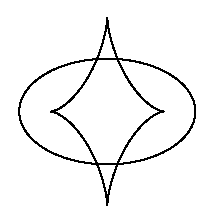
\includegraphics{asy/ellipse-astroid}
\vskip-0mm
\end{wrapfigure}

The curve $s\mapsto \omega(s)$ is called the \index{evolute}\emph{evolute} of $\gamma$; 
it traces the centers of curvature of the curve. 
The evolute of $\gamma$ can be written as 
\[\omega(t)=\gamma(t)+\tfrac1{\skur(t)}\cdot \norm(t)\] and  
in the proof we showed that $(\tfrac1{\skur})'\cdot\norm$ is its velocity vector.


\begin{thm}{Exercise}\label{ex:evolute-of-ellipse}
Show that the stretched astroid 
\[\omega(t)=(\tfrac{a^2-b^2}{a}\cdot \cos^3 t,  \tfrac{b^2-a^2}{b}\cdot\sin^3 t)\]
is an evolute of the ellipse defined by
\[\gamma(t)= (a\cdot \cos t, b\cdot\sin t).\]
\end{thm}

The following theorem states formally that 
\emph{if you drive on the plane and turn the steering wheel to the left all the time,
then you will not be able to come back to the place you started.}

}

\begin{thm}{Theorem}\label{thm:spiral}
Assume $\gamma$ is a smooth regular plane curve with positive and strictly monotonic signed curvature. 
Then $\gamma$ is simple.
\end{thm}

The same statement holds true without assuming positivity of curvature; the proof requires only minor modifications.

\parit{Proof of \ref{thm:spiral}.}
Note that $\gamma(s)$ lies on the osculating circle $\sigma_s$ of $\gamma$ at $s$.
If $s_1\ne s_0$, then by lemma \ref{lem:spiral}, $\sigma_{s_0}$ does not intersect $\sigma_{s_1}$.
Therefore $\gamma(s_1)\ne \gamma(s_0)$,
hence the result.\qeds

\begin{thm}{Exercise}\label{ex:3D-spiral}
Show that a 3-dimensional analog of the theorem does not hold.
That is, there are self-intersecting smooth regular space curves with strictly monotonic curvature.
\end{thm}

\begin{thm}{Exercise}\label{ex:double-tangent}
Assume that $\gamma$ is a smooth regular plane curve with positive strictly monotonic signed curvature.

\begin{subthm}{ex:double-tangent:a}Show that no line can be tangent to $\gamma$ at two distinct points.
\end{subthm}

\begin{subthm}{ex:double-tangent:b}Show that no circle can be tangent to $\gamma$ at three distinct points. 
\end{subthm}

\end{thm}

{

\begin{wrapfigure}{o}{35 mm}
\vskip-4mm
\centering
\includegraphics{mppics/pic-25}
\vskip0mm
\end{wrapfigure}

Note that part \ref{SHORT.ex:double-tangent:a} does not hold if we allow the curvature to be negative; an example is shown on the diagram.

}



